\section{First Experimental Tests}

In polarized deep inelastic scattering, a longitudinally polarized lepton beam is scattered off of nucleon targets polarized parallel or perpendicular to the beam axis. Asymmetries are formed by comparing event rates for scattering in different spin configurations.  For a spin $\frac{1}{2}$ target, the asymmetries of interest are

% Stiegler does not include the 1/2 nor the differential in this equation
\begin{equation}
  A_{\parallel} = \frac{d\sigma^{\rightarrow \Leftarrow} - d\sigma^{\rightarrow \Rightarrow}}{2d\sigma_{unpol}}, ~~~~~~~
  A_{\perp} = \frac{d\sigma^{\rightarrow \Uparrow} - d\sigma^{\rightarrow \Downarrow}}{2d\sigma_{unpol}}
\end{equation}

Spin-dependent cross sections can be calculated by contracting the elastic Compton amplitude $T_{\mu \nu}$ with the photon polarization vectors; in the presence of parity conservation and time reversal, four of these are independent \cite{??}:
%
\begin{eqnarray}
  \sigma_{1/2} & = & F_1 + g_1 - \gamma^2 g_2, \nonumber \\
  \sigma_{3/2} & = & F_1 - g_1 + \gamma^2 g_2, \nonumber \\
  \sigma_L & = & -F_1 + F_2(1+\gamma^2)/(2x),  \nonumber \\
  \sigma_{TL} & = & \sqrt{2}\gamma (g_1+g_2).
\end{eqnarray}
%
Here $\gamma^2 = Q^2/v^2$.  These four cross sections are commonly rearranged into a pair of virtual photon asymmetries $A_1$ and $A_2$:
%
\begin{equation}
  A_1 = \frac{\sigma_{1/2} - \sigma_{3/2}}{\sigma_{1/2} - \sigma_{3/2}}, ~~~~ A_2 = \frac{\sigma_{TL}}{\sigma_T}
\end{equation}
%
The longitudinal and transverse DIS asymmetries can then be written in terms of these virtual photon asymmetries,
\begin{equation}
  A_{\parallel} = D(A_1 + \eta A_2), ~~~~~ A_{\perp} = d(A_2 - \xi A_1)
\end{equation}
%
where the coefficients $D$, $\eta$, $d$, and $\xi$ can be approximated to first order in $\gamma$ in terms of the usual DIS kinematic variables and $R = \frac{\sigma_{TL}}{\sigma_T}$:
\begin{eqnarray}
  D & \approx & \frac{y(2-y)}{y^2 + 2(1-y)(1+R)}, ~~~~~~~~ \eta \approx \frac{2(1-y)}{y(2-y)} \frac{\sqrt{Q^2}}{E} \nonumber \\
  d & \approx & D \frac{\sqrt{1-y}}{1-y/2}, ~~~~~~~~ \xi \approx \gamma(1-\frac{y}{2})
\end{eqnarray}
%
$D$ can be thought of as a depolarization factor arising from the fact that the photon is not fully aligned with the lepton beam, and $\eta$, $\xi$ are kinematic factors that are usually small.  The structure functions can also be written in terms of $A_{1,2}$:
\begin{equation}
  g_1 = \frac{F_2}{2x(1+R)}(A_1+\gamma A_2), ~~~~~ g_2 = \frac{F_2}{2x(1+R)}(A_2/\gamma - A_1).
\end{equation}
Thus, measurements of $A_{\parallel}$, $A_{\perp}$, $F_2$, and $R$ are sufficient to extract the polarized structure functions of the nucleon.

% \begin{equation}
%   \gamma = \sqrt{\frac{2Mx}{Ey}}
% \end{equation}

% note that they just measured A_parallel and neglected the A_2 contribution
The first DIS experiments to extract $g_1$ were E80 and E130, conducted in the early 1980s at SLAC.  These experiments scattered longitudinally polarized electron beams off of longitudinally polarized proton targets and were able to measure $A_1^p$ in the range $0.1 < x < 0.7$.  Their results were consistent with expectations from the parton model in that limited kinematic regime.

In 1988, the European Muon Collaboration (EMC) published data on asymmetries of longitudinally polarized \textit{muon} beams scattering off of longitudinally polarized proton targets.  

From these data they extracted measurements of the proton's $g_1$ structure function over a wide range in $x$ and $Q^2$.  As shown in Figure \ref{fig:emc-g1p}, the integral value of $g_1^p$ obtained from that extraction was incompatible with the prediction from Ellis and Jaffe.

% measured asymmetry


\begin{equation}
  A_1 = (g_1 - \gamma^2 g_2)\frac{1}{F_1}, ~~~~~~~~ A_2 = \gamma(g_1+g_2)\frac{1}{F_1}
\end{equation}

\begin{figure}
  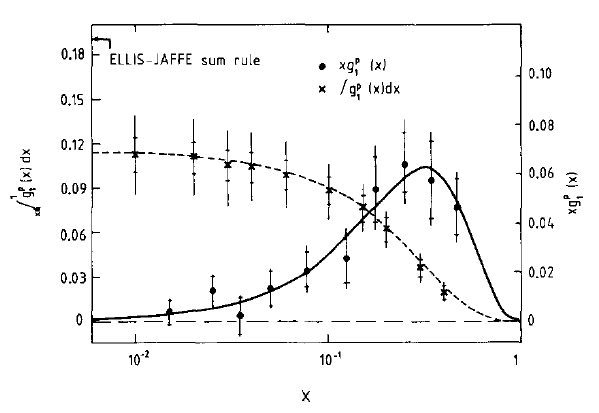
\includegraphics[width=1.0\textwidth]{figures/emc-g1p}
  \caption{EMC extraction of $g^1_p$ and its integral compared to the prediction from Ellis-Jaffe \cite{Ashman:1987hv}}
  \label{fig:emc-g1p}
\end{figure}

\begin{equation}
  A_1 \approx \frac{A_{\parallel}}{D} \approx (1 + \gamma^2)\frac{g_1}{F_1}
\end{equation}

EMC measures first moment of g1, taking a3 and a8 from beta-decay measurements means that we can extract a0 from $\Gamma_1^p$ and it's $\sim$ 0.  But

\begin{equation}
  a_0 = \Delta \Sigma = a_8 + 3(\Delta s + \Delta \bar{s})
\end{equation}

from above, and if you ignore strange quark contributions (Ellis-Jaffe) you get $a_0 \sim 0.59$, obviously in stark contrast to EMC.  This is the original ``spin crisis''.  And of course $a_0 = 2<S_z^{quarks}>$.

Any need to mention ``Cloudy Bag'' model here?  I think not.

Detailed derivation of these results can be found in \cite{Anselmino:1994gn}

\begin{equation}
  y \equiv \frac{\nu}{E} = \frac{P \cdot q}{P \cdot k}
\end{equation}

\begin{equation}
  \gamma^2 = \frac{4M^2x^2}{Q^2}
\end{equation}
